\documentclass[11pt,a4paper]{article}
\usepackage[utf8]{inputenc}
\usepackage[T1]{fontenc}
\usepackage{amsmath,amssymb}
\usepackage{geometry,enumitem,booktabs,xcolor}
\usepackage{tcolorbox}
\usepackage{tikz}
\usetikzlibrary{arrows.meta,positioning,calc,decorations.pathreplacing,mindmap,shapes.geometric}
\usepackage{hyperref}
\usepackage{longtable}

\geometry{margin=2cm}
\hypersetup{colorlinks=true,linkcolor=blue!60!black,urlcolor=blue!70!black,citecolor=green!50!black}
\tcbuselibrary{skins}

\definecolor{discover}{HTML}{2E86AB}
\definecolor{physics}{HTML}{A23B72}
\definecolor{symbolic}{HTML}{F18F01}
\definecolor{structure}{HTML}{2CA58D}
\definecolor{foundation}{HTML}{7B2D8E}

\title{\textbf{Literature Review}\\[4pt]
\Large Scientific Discovery via Artificial Intelligence\\[4pt]
\large From Physics-Informed Networks to Automated Structure Discovery\\[6pt]
\normalsize Starting Point: $\Psi$-NN (Liu et al., \textit{Nature Communications}, 2025)}
\author{PFE -- Meeting 3}
\date{\today}

\begin{document}
\maketitle

\begin{abstract}
\noindent This literature review maps the emerging field of \textbf{scientific discovery via AI}, moving beyond using AI as a black-box tool toward AI that \emph{discovers} physical laws, symmetries, equations, and structures autonomously. The $\Psi$-NN paper (Liu et al., 2025) serves as our entry point, situated at the intersection of physics-informed learning, knowledge distillation, and automatic symmetry discovery. We organize the field into six major research axes, identify seminal works in each, and highlight open problems and connections.
\end{abstract}

\tableofcontents
\newpage

%=================================================================
\section{Landscape of the Field}
%=================================================================

\begin{center}
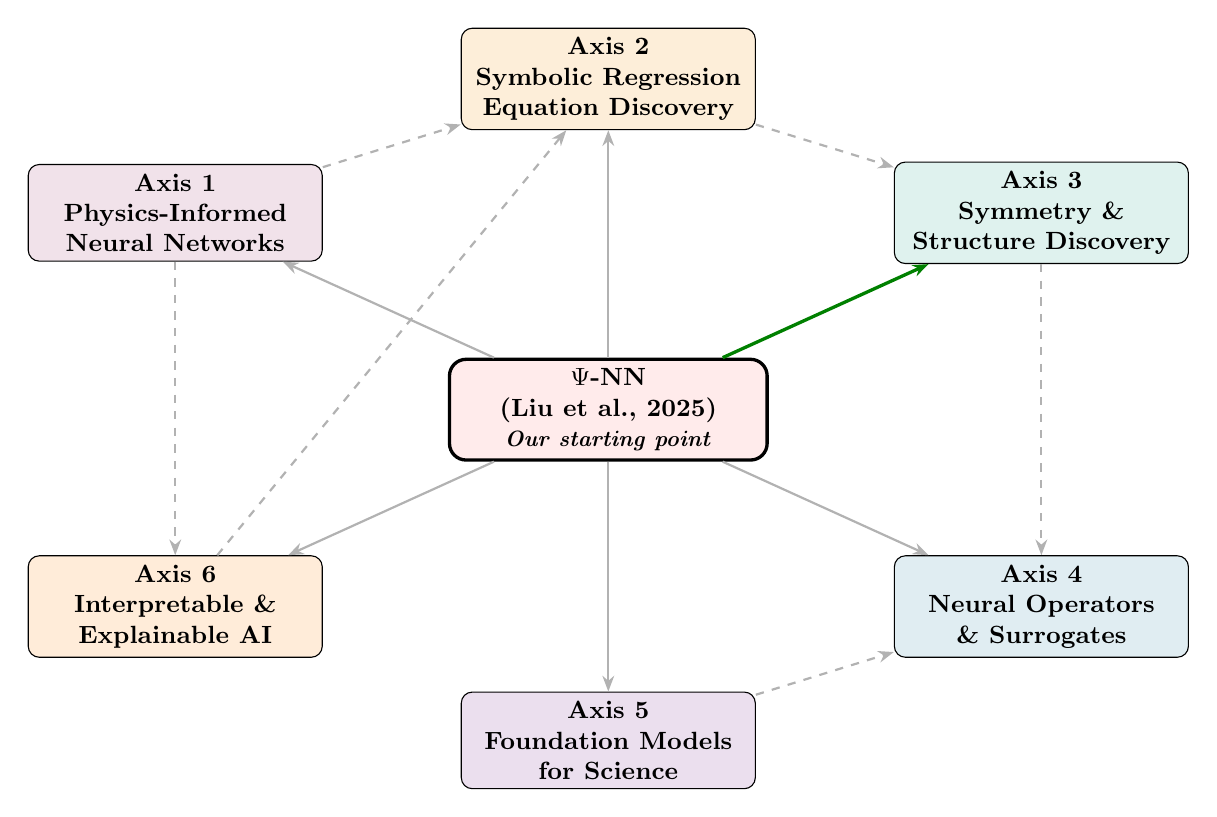
\begin{tikzpicture}[
    every node/.style={font=\small},
    axis/.style={draw,rounded corners=4pt,minimum height=1.1cm,text width=3.5cm,align=center,font=\small\bfseries},
    link/.style={-{Stealth[length=2mm]},thick,gray!60},
    entry/.style={draw,rounded corners=6pt,very thick,minimum height=1.2cm,text width=3.8cm,align=center,fill=red!8,font=\small\bfseries}
]
% Center: entry point
\node[entry] (psi) {$\Psi$-NN\\(Liu et al., 2025)\\{\footnotesize\textit{Our starting point}}};

% Six axes
\node[axis,fill=physics!15]   (ax1) at (-5.5, 2.5) {Axis 1\\Physics-Informed\\Neural Networks};
\node[axis,fill=symbolic!15]  (ax2) at (0, 4.2)     {Axis 2\\Symbolic Regression\\Equation Discovery};
\node[axis,fill=structure!15] (ax3) at (5.5, 2.5)   {Axis 3\\Symmetry \&\\Structure Discovery};
\node[axis,fill=discover!15]  (ax4) at (5.5,-2.5)   {Axis 4\\Neural Operators\\\& Surrogates};
\node[axis,fill=foundation!15](ax5) at (0,-4.2)     {Axis 5\\Foundation Models\\for Science};
\node[axis,fill=orange!15]    (ax6) at (-5.5,-2.5)  {Axis 6\\Interpretable \&\\Explainable AI};

\draw[link] (psi) -- (ax1);
\draw[link] (psi) -- (ax2);
\draw[link,very thick,green!50!black] (psi) -- (ax3);
\draw[link] (psi) -- (ax4);
\draw[link] (psi) -- (ax5);
\draw[link] (psi) -- (ax6);

% Cross-links
\draw[link,dashed] (ax1) -- (ax2);
\draw[link,dashed] (ax2) -- (ax3);
\draw[link,dashed] (ax3) -- (ax4);
\draw[link,dashed] (ax1) -- (ax6);
\draw[link,dashed] (ax5) -- (ax4);
\draw[link,dashed] (ax6) -- (ax2);
\end{tikzpicture}
\end{center}

\begin{tcolorbox}[colback=red!3,colframe=red!50!black,title={\small Key Insight: What Makes This ``Discovery'' Not Just ``Application''?}]
\small
\textbf{Application:} Train a neural network to approximate a known PDE solution.\\
\textbf{Discovery:} The AI \emph{finds} the equation, symmetry, or structure that was previously unknown.\\[3pt]
$\Psi$-NN sits at this boundary: it takes a known PDE but \textbf{discovers} hidden structural symmetries in the solution space that even the human expert didn't encode.
\end{tcolorbox}

%=================================================================
\section{Axis 1: Physics-Informed Neural Networks (PINNs)}
%=================================================================

\subsection{Foundation}

\begin{center}
\renewcommand{\arraystretch}{1.3}
\begin{tabular}{@{}p{3.5cm} p{4cm} p{5.5cm}@{}}
\toprule
\textbf{Paper} & \textbf{Key Contribution} & \textbf{Relevance to Discovery} \\
\midrule
Raissi, Perdikaris \& Karniadakis (2019) \textit{J.\ Comput.\ Phys.} & Introduced PINNs: embed PDEs into neural network loss & Foundation layer; physics as soft constraint only \\
\addlinespace
Lagaris et al.\ (1998) \textit{IEEE Trans.\ NN} & Early physics-constrained NNs for ODEs/PDEs & Historical precursor; hard boundary constraints \\
\addlinespace
Lu et al.\ (2021) \textit{SIAM Review} & DeepXDE framework; residual-based adaptive refinement & Practical toolkit; scalable PINNs \\
\bottomrule
\end{tabular}
\end{center}

\subsection{Key limitations that motivate discovery}

\begin{enumerate}[leftmargin=1.8em,itemsep=2pt]
\item \textbf{Soft constraint only:} PDE is in the loss $\Rightarrow$ no guarantee of satisfaction.
\item \textbf{Spectral bias:} NNs learn low-frequency components first $\Rightarrow$ poor on multi-scale problems.
\item \textbf{Training difficulty:} Balancing PDE loss vs.\ boundary loss vs.\ data loss.
\item \textbf{No structural awareness:} The network doesn't ``know'' about symmetries, conservation laws, etc.
\end{enumerate}

$\Rightarrow$ These limitations drive the need for methods that go beyond PINNs: discovering and embedding structure.

\subsection{Extensions toward discovery}

\begin{center}
\renewcommand{\arraystretch}{1.25}
\begin{tabular}{@{}p{4cm} p{3.5cm} p{5.5cm}@{}}
\toprule
\textbf{Paper} & \textbf{Method} & \textbf{Discovery Aspect} \\
\midrule
Wang et al.\ (2021) \textit{SIAM J.\ Sci.\ Comput.} & NTK-based loss balancing & Discovers optimal training dynamics \\
Jagtap \& Karniadakis (2020) & Adaptive activation functions & Network discovers best nonlinearity \\
McClenny \& Brainerd (2023) & Self-adaptive PINNs & Discovers where physics is hard to satisfy \\
\textbf{Liu et al.\ (2025)} & \textbf{$\Psi$-NN} & \textbf{Discovers symmetry structure in weights} \\
\bottomrule
\end{tabular}
\end{center}

%=================================================================
\section{Axis 2: Symbolic Regression \& Equation Discovery}
%=================================================================

\textbf{Goal:} Given data, find the \emph{closed-form equation} that generated it.

\subsection{Seminal methods}

\begin{center}
\renewcommand{\arraystretch}{1.3}
\begin{tabular}{@{}p{3.5cm} p{3cm} p{3cm} p{3cm}@{}}
\toprule
\textbf{Paper} & \textbf{Method} & \textbf{Approach} & \textbf{Key Result} \\
\midrule
Schmidt \& Lipson (2009) \textit{Science} & Eureqa & Genetic programming & Rediscovered Newton's laws from data \\
\addlinespace
Brunton et al.\ (2016) \textit{PNAS} & SINDy & Sparse regression on library of functions & Discovers governing ODEs/PDEs from time-series \\
\addlinespace
Udrescu \& Tegmark (2020) \textit{Sci.\ Advances} & AI Feynman & Neural net + symbolic simplification & Rediscovered 100 physics equations from Feynman Lectures \\
\addlinespace
Cranmer (2023) & PySR & Optimized genetic programming with regularization & Open-source state-of-the-art symbolic regression \\
\addlinespace
Long et al.\ (2018) \textit{ICML} & PDE-Net & CNN learns PDE coefficients & Discovers PDE form from spatiotemporal data \\
\bottomrule
\end{tabular}
\end{center}

\subsection{Connection to $\Psi$-NN}

\begin{tcolorbox}[colback=symbolic!5,colframe=symbolic!70!black]
\small
\textbf{SINDy/AI Feynman} discover the \emph{equation} from data.\\
\textbf{$\Psi$-NN} discovers the \emph{structural symmetries of the solution} given the equation.\\[3pt]
They are complementary: one works upstream (what is the PDE?), the other downstream (what structure does the PDE impose on the solution?). A full pipeline would chain both.
\end{tcolorbox}

\subsection{Recent advances}

\begin{itemize}[leftmargin=1.8em,itemsep=2pt]
\item \textbf{Symbolic GPT} (Biggio et al., 2021): Transformer trained to output symbolic expressions from numerical data.
\item \textbf{E2E Symbolic Regression} (Kamienny et al., 2022, \textit{NeurIPS}): End-to-end transformer for symbolic regression.
\item \textbf{$\Phi$-SO} (Tenachi et al., 2023, \textit{NeurIPS}): Physical Symbolic Optimization -- uses dimensional analysis to constrain the search.
\item \textbf{LLM-SR} (Shojaee et al., 2024): Uses LLMs to propose and refine symbolic expressions.
\end{itemize}

%=================================================================
\section{Axis 3: Symmetry \& Structure Discovery}
%=================================================================

This is the axis where $\Psi$-NN sits. The goal: \textbf{automatically find symmetries, invariances, and conservation laws from data or models}.

\subsection{Taxonomy}

\begin{center}
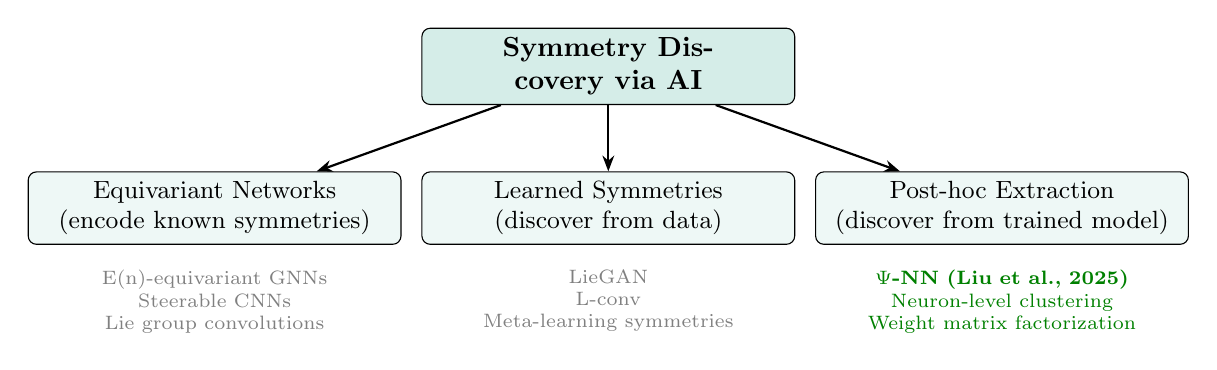
\begin{tikzpicture}[
    every node/.style={font=\small},
    cat/.style={draw,rounded corners=3pt,minimum height=0.8cm,text width=4.5cm,align=center,fill=structure!8},
    arr/.style={-{Stealth[length=2mm]},thick}
]
\node[cat,fill=structure!20,font=\bfseries] (root) at (0,0) {Symmetry Discovery via AI};
\node[cat] (eq) at (-5,-1.8) {Equivariant Networks\\(encode known symmetries)};
\node[cat] (learn) at (0,-1.8) {Learned Symmetries\\(discover from data)};
\node[cat] (extract) at (5,-1.8) {Post-hoc Extraction\\(discover from trained model)};
\draw[arr] (root) -- (eq);
\draw[arr] (root) -- (learn);
\draw[arr] (root) -- (extract);

\node[below=0.2cm of eq,font=\scriptsize,gray,text width=4.5cm,align=center] {E(n)-equivariant GNNs\\Steerable CNNs\\Lie group convolutions};
\node[below=0.2cm of learn,font=\scriptsize,gray,text width=4.5cm,align=center] {LieGAN\\L-conv\\Meta-learning symmetries};
\node[below=0.2cm of extract,font=\scriptsize,text width=4.5cm,align=center,green!50!black] {\textbf{$\Psi$-NN (Liu et al., 2025)}\\Neuron-level clustering\\Weight matrix factorization};
\end{tikzpicture}
\end{center}

\subsection{Key papers}

\begin{center}
\renewcommand{\arraystretch}{1.3}
\begin{tabular}{@{}p{3.8cm} p{3.5cm} p{5.2cm}@{}}
\toprule
\textbf{Paper} & \textbf{What It Discovers} & \textbf{How} \\
\midrule
Cohen \& Welling (2016) \textit{ICML} & Group equivariant CNNs & Encodes known symmetries in convolution filters \\
\addlinespace
Weiler et al.\ (2018) & Steerable CNNs & General $E(2)$-equivariance via steerable filters \\
\addlinespace
Satorras et al.\ (2021) \textit{ICML} & E(n) Equivariant GNNs (EGNN) & SE(3)-equivariant graph nets for molecules \\
\addlinespace
\textbf{Moskalev et al.\ (2022)} \textit{NeurIPS} & \textbf{LieGAN} & \textbf{GAN discovers Lie group symmetries from data} \\
\addlinespace
Yang et al.\ (2023) & Generative symmetry discovery & Learns continuous symmetry transformations \\
\addlinespace
Desai et al.\ (2022) & Symmetry discovery from equation form & Symbolic computation of Lie symmetries \\
\addlinespace
\textbf{Liu et al.\ (2025)} & \textbf{$\Psi$-NN} & \textbf{Distillation $\to$ clustering $\to$ relation matrix $\R$} \\
\bottomrule
\end{tabular}
\end{center}

\subsection{What $\Psi$-NN adds to this axis}

\begin{tcolorbox}[colback=structure!5,colframe=structure!70!black,title={\small $\Psi$-NN's unique contribution}]
\small
\begin{itemize}[leftmargin=1.2em,itemsep=1pt]
\item Most equivariant methods \textbf{encode known} symmetries. $\Psi$-NN \textbf{discovers unknown} ones.
\item Unlike LieGAN (which works in data space), $\Psi$-NN works in \textbf{weight space}.
\item The relation matrix $\mathbf{R}$ is \textbf{interpretable}: each entry maps to a physical symmetry (sharing, sign flip, permutation).
\item Limitation: currently restricted to discrete sign/permutation symmetries, not continuous Lie groups.
\end{itemize}
\end{tcolorbox}

%=================================================================
\section{Axis 4: Neural Operators \& Learned Surrogates}
%=================================================================

\textbf{Goal:} Learn the \emph{solution operator} $\mathcal{G}: f \mapsto u$ (function-to-function mapping), not just one solution.

\subsection{Key architectures}

\begin{center}
\renewcommand{\arraystretch}{1.3}
\begin{tabular}{@{}p{3.5cm} p{3.5cm} p{5.5cm}@{}}
\toprule
\textbf{Paper} & \textbf{Architecture} & \textbf{Discovery Potential} \\
\midrule
Lu et al.\ (2021) \textit{Nature Mach.\ Intell.} & DeepONet & Universal operator approximation; can learn unknown operators from data \\
\addlinespace
Li et al.\ (2021) \textit{ICLR} & Fourier Neural Operator (FNO) & Learns in spectral space; resolution-invariant; captures multi-scale physics \\
\addlinespace
Kovachki et al.\ (2023) & Neural Operator survey & Unifying framework for all operator learning methods \\
\addlinespace
Hao et al.\ (2023) & GNOT & General neural operator transformer; attention-based \\
\addlinespace
Brandstetter et al.\ (2022) & Message-passing neural PDE solver & GNN-based; learns update rules \\
\bottomrule
\end{tabular}
\end{center}

\subsection{Connection to discovery}

Neural operators can discover:
\begin{itemize}[leftmargin=1.8em,itemsep=2pt]
\item \textbf{Unknown governing operators} from input-output data pairs.
\item \textbf{Closure models} for unresolved physics (turbulence, subgrid).
\item \textbf{Constitutive laws} in multiphysics problems.
\end{itemize}

Combining neural operators with $\Psi$-NN's structure discovery: a neural operator that \textbf{also reveals the symmetries} of the operator it learned $\Rightarrow$ open research direction.

%=================================================================
\section{Axis 5: Foundation Models for Science}
%=================================================================

\textbf{Goal:} Large pre-trained models that transfer across scientific tasks, analogous to GPT/BERT in NLP.

\subsection{Landmark systems}

\begin{center}
\renewcommand{\arraystretch}{1.3}
\begin{tabular}{@{}p{3.5cm} p{3cm} p{6cm}@{}}
\toprule
\textbf{System} & \textbf{Domain} & \textbf{Discovery} \\
\midrule
AlphaFold 2 (Jumper et al., 2021, \textit{Nature}) & Protein structure & Predicted 3D structure of \textasciitilde200M proteins; Nobel Prize 2024 \\
\addlinespace
GNoME (Merchant et al., 2023, \textit{Nature}) & Materials science & Discovered 2.2M new stable crystal structures \\
\addlinespace
Galactica (Taylor et al., 2022) & Scientific text & LLM trained on 48M scientific papers \\
\addlinespace
FourCastNet (Pathak et al., 2022) & Weather & FNO-based global weather forecasting \\
\addlinespace
GenCast (Price et al., 2024, \textit{Nature}) & Weather & Diffusion-based probabilistic weather prediction \\
\addlinespace
MACE-MP-0 (Batatia et al., 2024) & Molecular dynamics & Universal interatomic potential for the periodic table \\
\bottomrule
\end{tabular}
\end{center}

\subsection{Relevance}

These systems show AI can make \textbf{genuine scientific discoveries} at scale. The key pattern:
\begin{enumerate}[leftmargin=1.8em,itemsep=2pt]
\item Pre-train on massive scientific data.
\item Embed physical constraints (symmetry, conservation) into architecture.
\item Generate predictions beyond known data $\Rightarrow$ discovery.
\end{enumerate}

$\Psi$-NN's approach (auto-discovering structure) could augment step 2: instead of hand-designing equivariant architectures, let the model discover what symmetries to embed.

%=================================================================
\section{Axis 6: Interpretable \& Explainable AI for Science}
%=================================================================

\textbf{Goal:} Not just accurate predictions, but \emph{understanding} what the model learned -- extracting scientific insight.

\subsection{Key approaches}

\begin{center}
\renewcommand{\arraystretch}{1.3}
\begin{tabular}{@{}p{3.5cm} p{3cm} p{6cm}@{}}
\toprule
\textbf{Method} & \textbf{Type} & \textbf{Scientific Insight Extracted} \\
\midrule
SHAP (Lundberg \& Lee, 2017) & Post-hoc feature attribution & Which input features matter for each prediction \\
\addlinespace
Concept Bottleneck Models (Koh et al., 2020) & Interpretable by design & Maps to human-defined scientific concepts \\
\addlinespace
Sparse autoencoders (Cunningham et al., 2023) & Mechanistic interpretability & Discovers interpretable features in hidden layers \\
\addlinespace
Neural additive models (Agarwal et al., 2021) & Inherently interpretable & Learns additive decomposition of effects \\
\addlinespace
\textbf{$\Psi$-NN (Liu et al., 2025)} & \textbf{Post-hoc structure extraction} & \textbf{Relation matrix $\mathbf{R}$ maps to physical symmetries} \\
\bottomrule
\end{tabular}
\end{center}

\subsection{Why interpretability matters for discovery}

\begin{tcolorbox}[colback=orange!3,colframe=orange!60!black]
\small A black-box AI that achieves 99\% accuracy is an \textbf{application tool}. An AI whose internal representations can be read as physical laws is a \textbf{discovery tool}. The $\Psi$-NN relation matrix is a step toward the latter: the structure of $\mathbf{R}$ directly corresponds to symmetries of the PDE.
\end{tcolorbox}

%=================================================================
\section{Synthesis: How $\Psi$-NN Connects the Axes}
%=================================================================

\begin{center}
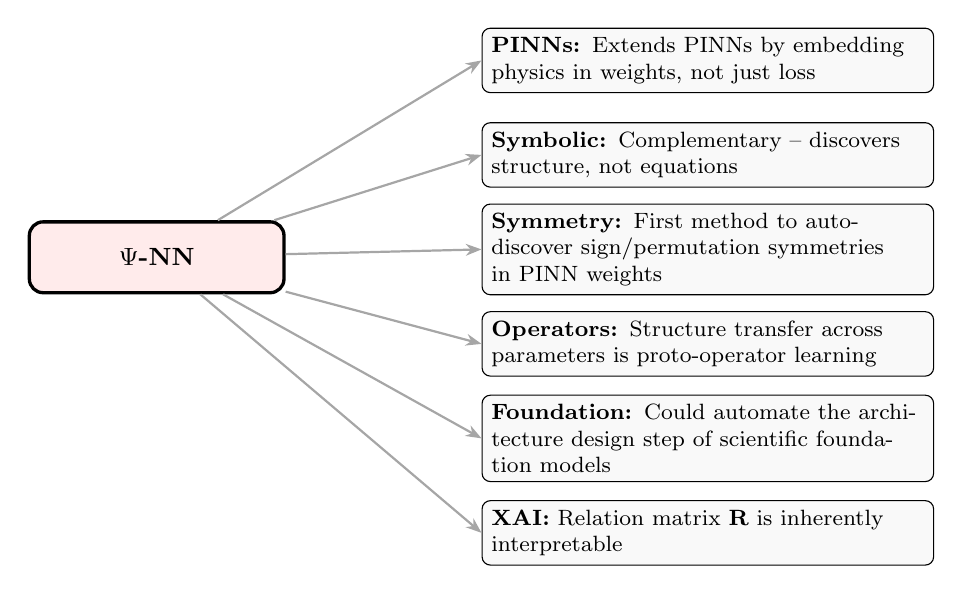
\begin{tikzpicture}[
    every node/.style={font=\footnotesize},
    psi/.style={draw,very thick,rounded corners=5pt,fill=red!8,minimum height=0.9cm,text width=3cm,align=center,font=\small\bfseries},
    conn/.style={draw,rounded corners=3pt,fill=gray!5,minimum height=0.7cm,text width=5.5cm,align=left,font=\footnotesize},
    arr/.style={-{Stealth[length=2mm]},thick,gray!70}
]
\node[psi] (psi) at (0,0) {$\Psi$-NN};

\node[conn] (c1) at (7, 2.5) {\textbf{PINNs:} Extends PINNs by embedding physics in weights, not just loss};
\node[conn] (c2) at (7, 1.3) {\textbf{Symbolic:} Complementary -- discovers structure, not equations};
\node[conn] (c3) at (7, 0.1) {\textbf{Symmetry:} First method to auto-discover sign/permutation symmetries in PINN weights};
\node[conn] (c4) at (7,-1.1) {\textbf{Operators:} Structure transfer across parameters is proto-operator learning};
\node[conn] (c5) at (7,-2.3) {\textbf{Foundation:} Could automate the architecture design step of scientific foundation models};
\node[conn] (c6) at (7,-3.5) {\textbf{XAI:} Relation matrix $\mathbf{R}$ is inherently interpretable};

\draw[arr] (psi) -- (c1.west);
\draw[arr] (psi) -- (c2.west);
\draw[arr] (psi) -- (c3.west);
\draw[arr] (psi) -- (c4.west);
\draw[arr] (psi) -- (c5.west);
\draw[arr] (psi) -- (c6.west);
\end{tikzpicture}
\end{center}

%=================================================================
\section{Open Problems \& Future Directions}
%=================================================================

\begin{center}
\renewcommand{\arraystretch}{1.4}
\begin{tabular}{@{}c p{5cm} p{6.5cm}@{}}
\toprule
\textbf{\#} & \textbf{Open Problem} & \textbf{Why It Matters} \\
\midrule
1 & Extend $\Psi$-NN to continuous symmetries (rotations, Lie groups) & Current method limited to sign flips and permutations \\
2 & Apply structure discovery to Transformers / attention architectures & $\Psi$-NN validated only on 3-layer MLP + $\tanh$ \\
3 & End-to-end pipeline: data $\to$ equation $\to$ structure $\to$ constrained solver & Combine SINDy/AI Feynman + $\Psi$-NN + neural operator \\
4 & Discover conservation laws, not just symmetries & Noether's theorem links symmetries to conserved quantities \\
5 & Scale to high-dimensional PDEs (100+ dimensions) & Current benchmarks are 2D--3D \\
6 & Foundation model for PDE structure & Pre-train on many PDEs, transfer discovered structures \\
7 & Formal verification of discovered symmetries & Currently empirical; need mathematical guarantees \\
8 & Discover symmetry breaking & Many physical systems have approximate or broken symmetries \\
\bottomrule
\end{tabular}
\end{center}

%=================================================================
\section{Suggested Reading Plan}
%=================================================================

Organized from foundational to advanced, prioritized for the PFE direction.

\subsection{Tier 1: Must-read (core foundation)}

\begin{enumerate}[leftmargin=1.8em,itemsep=3pt]
\item \textbf{Raissi et al.} (2019) -- PINNs. \textit{J.\ Comput.\ Phys.} 378, 686--707.
\item \textbf{Liu et al.} (2025) -- $\Psi$-NN. \textit{Nature Communications} 16, 9558. \textcolor{red}{$\star$ Our starting paper.}
\item \textbf{Brunton et al.} (2016) -- SINDy. \textit{PNAS} 113(15), 3932--3937.
\item \textbf{Udrescu \& Tegmark} (2020) -- AI Feynman. \textit{Science Advances} 6(16).
\item \textbf{Li et al.} (2021) -- Fourier Neural Operator. \textit{ICLR}.
\end{enumerate}

\subsection{Tier 2: Important (symmetry \& structure focus)}

\begin{enumerate}[leftmargin=1.8em,itemsep=3pt]
\setcounter{enumi}{5}
\item \textbf{Moskalev et al.} (2022) -- LieGAN: symmetry discovery with GANs. \textit{NeurIPS}.
\item \textbf{Cohen \& Welling} (2016) -- Group equivariant CNNs. \textit{ICML}.
\item \textbf{Satorras et al.} (2021) -- E(n) Equivariant GNNs. \textit{ICML}.
\item \textbf{Long et al.} (2018) -- PDE-Net. \textit{ICML}.
\item \textbf{Lu et al.} (2021) -- DeepONet. \textit{Nature Machine Intelligence} 3, 218--229.
\end{enumerate}

\subsection{Tier 3: Broader landscape}

\begin{enumerate}[leftmargin=1.8em,itemsep=3pt]
\setcounter{enumi}{10}
\item \textbf{Jumper et al.} (2021) -- AlphaFold 2. \textit{Nature} 596, 583--589.
\item \textbf{Merchant et al.} (2023) -- GNoME. \textit{Nature} 624, 80--85.
\item \textbf{Cranmer} (2023) -- PySR: interpretable symbolic regression.
\item \textbf{Tenachi et al.} (2023) -- $\Phi$-SO: physics-aware symbolic optimization. \textit{NeurIPS}.
\item \textbf{Kovachki et al.} (2023) -- Neural Operator survey.
\end{enumerate}

%=================================================================
\section{Summary Table: Methods Comparison}
%=================================================================

\begin{center}
\small
\renewcommand{\arraystretch}{1.25}
\begin{tabular}{@{}l c c c c c@{}}
\toprule
\textbf{Method} & \textbf{Discovers} & \textbf{Needs PDE?} & \textbf{Interpretable?} & \textbf{Transferable?} & \textbf{Architecture} \\
\midrule
PINN & Nothing (solver) & Yes & No & No & MLP \\
SINDy & Equations & No (data only) & Yes & N/A & Sparse regression \\
AI Feynman & Equations & No (data only) & Yes & N/A & NN + symbolic \\
PDE-Net & PDE coefficients & Partial & Partial & No & CNN \\
FNO & Operator & No & No & Yes & Fourier layers \\
DeepONet & Operator & No & No & Yes & Branch-trunk \\
LieGAN & Lie symmetries & No & Yes & No & GAN \\
E(n)-GNN & Encodes symmetry & Known sym.\ & Yes & Yes & GNN \\
\textbf{$\Psi$-NN} & \textbf{Weight structure} & \textbf{Yes} & \textbf{Yes} & \textbf{Yes} & \textbf{MLP} \\
\bottomrule
\end{tabular}
\end{center}

%=================================================================
\section{Conclusion}
%=================================================================

The field of scientific discovery via AI is rapidly expanding beyond using neural networks as black-box function approximators. The $\Psi$-NN paper represents a concrete step in this direction: it shows that \textbf{physical structure can be automatically extracted from a trained neural network} and then \textbf{hard-coded back into the architecture}.

The broader research landscape connects six complementary axes:
\begin{itemize}[leftmargin=1.8em,itemsep=1pt]
\item PINNs provide the physics-informed foundation.
\item Symbolic regression discovers equations.
\item Symmetry discovery (where $\Psi$-NN contributes) finds structural constraints.
\item Neural operators learn solution mappings.
\item Foundation models scale discovery to new domains.
\item Interpretable AI ensures discovered knowledge is human-readable.
\end{itemize}

The most impactful future work likely lies at the \textbf{intersections}: combining equation discovery with structure discovery, scaling symmetry extraction to modern architectures (Transformers), and building foundation models that automatically discover and embed physical laws.

\end{document}
